\subsection{Introduction}
\begin{frame}{}
    \LARGE Autoencoders: \textbf{Introduction}
\end{frame}

\begin{frame}[allowframebreaks]{Autoencoders}
Autoencoders are a type of artificial neural network used for learning efficient codings of input data in an unsupervised manner. The goal is to learn a compressed (encoded) representation of the input and then reconstruct the original input from this compressed version.
\begin{itemize}
    \item \textbf{Developed originally in the 1980s}, autoencoders have gained renewed popularity due to advances in deep learning and hardware.
    \item Often used in \textbf{dimensionality reduction, denoising, anomaly detection, and generative modeling}.
\end{itemize}

\framebreak

\begin{itemize}
    \item Autoencoders are a family of neural networks designed to learn efficient representations of data, typically for dimensionality reduction or feature learning.
    \item They work by compressing the input into a latent-space representation (encoding), and then reconstructing the original input from this representation (decoding).
    \item The main goal is to project the input into a lower-dimensional latent space and then reconstruct the input from that latent representation.
\end{itemize}

\framebreak
    
Autoencoders consist of two main components:
\begin{itemize}
    \item \textbf{Encoder}: Maps the input data to a latent space $Z$, compressing the input into a lower-dimensional representation.
    \item \textbf{Decoder}: Reconstructs the input data from the encoded latent representation.
\end{itemize}

Variants of autoencoders may use altered or corrupted versions of the input as the target output, which can help the model learn more robust features (e.g., denoising autoencoders).

\framebreak

\begin{figure}
    \centering
    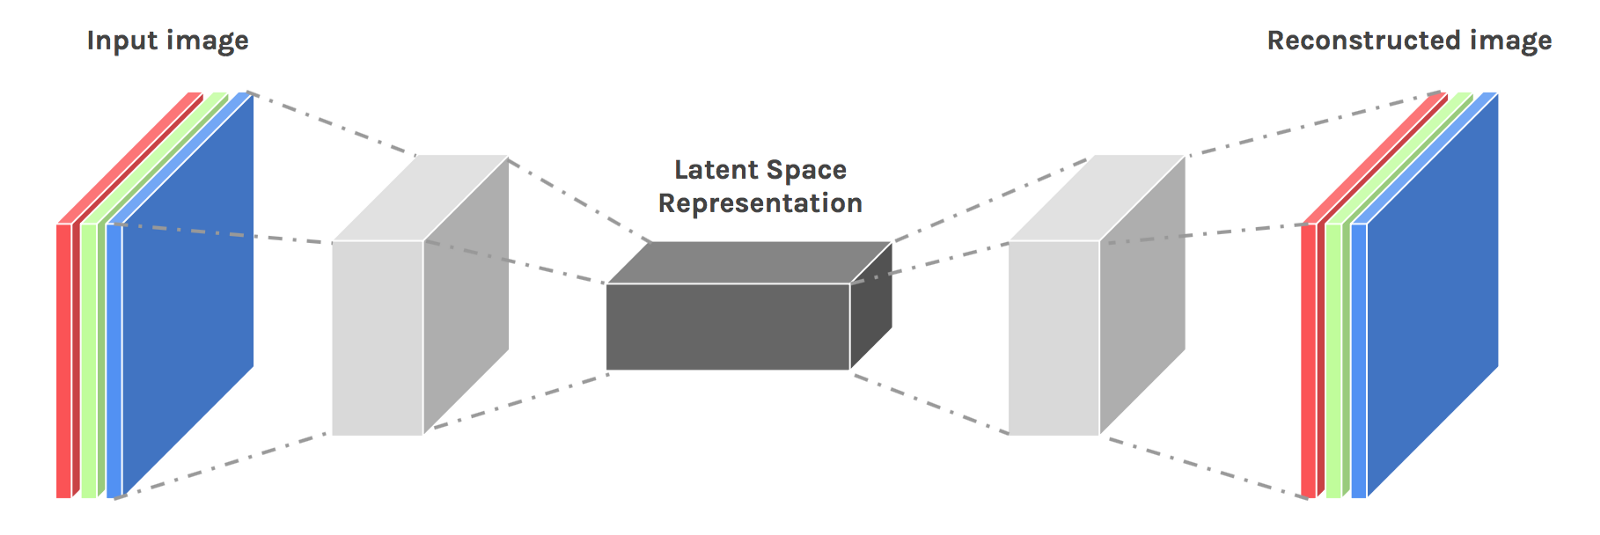
\includegraphics[height=\textheight, width=1.05\textwidth, keepaspectratio]{images/autoencoders/architecture.png}
    \caption*{Autoencoder architecture}
    \end{figure}

\framebreak

\begin{itemize}
    \setlength{\itemsep}{-0.2em}
        \item \textbf{Bottleneck (Latent Space)}
        \begin{itemize}
            \item The bottleneck is a small hidden layer in the middle of the network.
            \item It forces the network to squeeze the input into a shorter, simpler code.
            \item This helps the network find and keep only the most important information.
            \item A small bottleneck stops the autoencoder from just memorizing the input.
        \end{itemize}
        \item \textbf{Loss Function}
        \begin{itemize}
            \item Tells us how close the output is to the original input.
            \item The most common loss is \textbf{Mean Squared Error (MSE)}—it measures the average difference between input and output.
            \item For special cases, we can use other losses, like binary cross-entropy for yes/no data, or KL divergence for special types of autoencoders.
            \item The loss function guides the network to learn better and more useful features.
        \end{itemize}
\end{itemize}
\end{frame}